%
% codage SAT-OPEN
%
\subsection{Nouveau codage SAT dans les espaces de plans}

\fred{A ajouter: complexité en espace meilleure par rapport à MK99}

Les codages SAT dans les espaces de plans existants introduits par \cite{DBLP:conf/aaai/MaliK99} se r\'{e}f\`{e}rent tous \`{a} trois \'{e}tapes index\'{e}es (pas n\'{e}cessairement cons\'{e}cutives) du plan.
Dans notre nouveau codage, nous allons nous r\'{e}f\'{e}rer seulement \`{a} deux \'{e}tapes cons\'{e}cutives.
Pour chaque action $\a\in\A$ et chaque \'{e}tape $i$, nous cr\'{e}ons une variable propositionnelle $\a_{i}$ pour d\'{e}terminer qu'une instance de $\a$ doit \^{e}tre planifi\'{e}e \`{a} l'\'{e}tape $i$.
Pour chaque fluent $\f\in\F$ et chaque \'{e}tape $i$, nous cr\'{e}ons une variable propositionnelle $\open{\f}{i}$ pour exprimer que $\f$ se maintient \`{a} l'\'{e}tape pr\'{e}c\'{e}dente $i-1$ et doit \^{e}tre prot\'{e}g\'{e} au moins jusqu'\`{a} l'\'{e}tape $i$.

\begin{figure}[hb!]\centering
	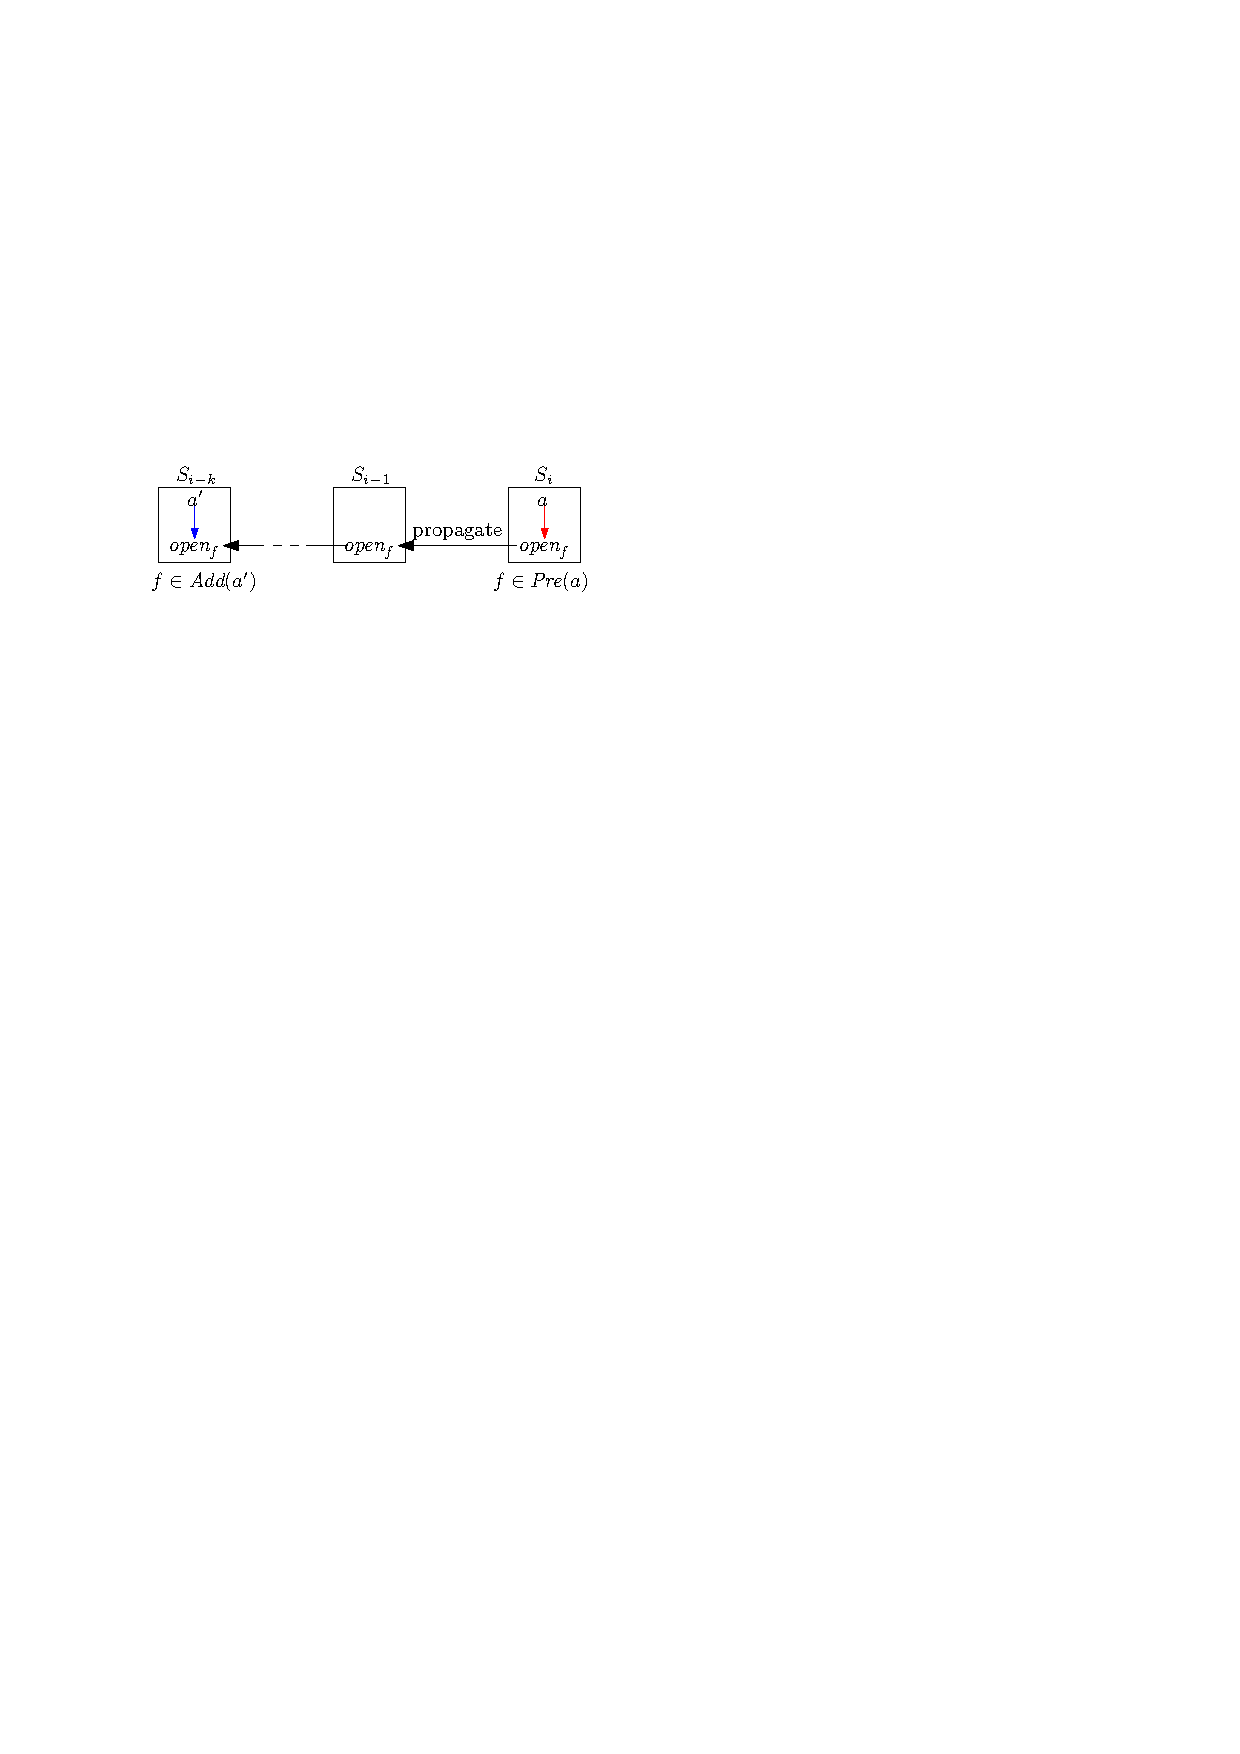
\includegraphics[width=.4\textwidth]{figures/transitions}
    \caption{Lien causal: l'action $a'$ produit $\f$ \`{a} l'\'{e}tape $S_{i-k}$ pour l'action $\a$ qui n\'{e}cessite $\f$ \`{a} l'\'{e}tape $S_{i}$.}
    \label{fig:causal-link-sat}
\end{figure}

Dans la figure~\ref{fig:causal-link-sat}, la variable $f$ est une \textit {condition ouverte} \`{a} l'\'{e}tape $\S_i$, impliquant que $\f\in\I$ ou une action $a'$ qui ajoute $\f$ est ex\'{e}cut\'{e}e dans une \'{e}tape pr\'{e}c\'{e}dente $\S_{i-k}$.
Les conditions ouvertes doivent \^{e}tre propag\'{e}es vers l'arri\`{e}re jusqu'\`{a} l'\'{e}tat initial ou une \'{e}tape dans laquelle elles sont ajout\'{e}es par une action.




%\paragraph*{SAT Encodings for Classical Planning}
%%\begin{figure}\label{steps:sat}
%%\begin{tiny}
%%%(a)\\[1em]
%%  \xymatrix@C=0.1pc@R=1pc{
%%  \text{S}_{0} (\textit{Init}) \ar@{>}[r] & \fbox{$x_{1}\equiv$ S$_{1}$} \ar@{>}[r]  & \fbox{$x_{2}\equiv$ S$_{2}$} \ar@{>}[r] & \fbox{$x_{3}\equiv$ S$_{3}$} \ar@{>}[r] & \fbox{$x_{4}\equiv$ S$_{4}$}
%%  \ar@{>}[r] & \fbox{$x_{5}\equiv$ S$_{5}$} \ar@{>}[r] & \fbox{$x_{6}\equiv$ S$_{6}$} \ar@{>}[r] & \fbox{$x_{7}\equiv$ S$_{7}$} \ar@{>}[r] & \text{S}_{8} (\textit{Goal}) \\
%%  }
%%\end{tiny}
%%%(b)\\[1em]
%%%   \hspace{0.8em}\xymatrix@C=0pc@R=1pc{
%%%   & & & & & \fbox{$x_{2}\equiv$ S$_{4}$} \ar@{.}[lld] \ar@{.}[rrd] \ar@/^1pc/[rdd] & & & & \\
%%%   & & & \fbox{$x_{1}\equiv$ S$_{2}$} \ar[rd] & & & & \fbox{$x_{1}\equiv$ S$_{6}$} \ar[rd] & & \\
%%%   \text{S}_{0} (\textit{Init}) \ar@{>}[rr] & & \fbox{$x_{0}\equiv$ S$_{1}$} \ar[ru]  & & \fbox{$x_{0}\equiv$ S$_{3}$} \ar@/^1pc/[ruu] & &  \fbox{$x_{0}\equiv$ S$_{5}$} \ar[ru] & & \fbox{$x_{0}\equiv$ S$_{7}$} \ar@{>}[rr] & & \text{S}_{8} (\textit{Goal}) \\
%%%  }
%%\vspace{1em}
%%\caption{Transitions of an 8-steps plan in SAT/SMT encoding}
%%\end{figure}
%  Each step $i$ is associated with:\hfill
%  \begin{itemize}
%    \item a set of propositional variables for actions $\{a_{i}^{1},a_{i}^{2}\ldots,a_{i}^{m}\}$
%    \item a set of propositional variables for open conditions $\{open_{f^1,i},open_{f^2,i},\ldots,open_{f^n,i}\}$ %which determine their value in state $x_{i-1}$
%  \end{itemize}


%\begin{frame}{SAT Encoding: open conditions}
%Given a propositional formula $\varphi$, $\textit{open}_{\varphi} = \textit{NNF}_{\textit{open}}(+1,\varphi)$ with:\\[0.8em]
%\begin{itemize}
%  \item $\textit{NNF}_{\textit{open}}(+1,f) = \textit{open}_{f}$
%  \item $\textit{NNF}_{\textit{open}}(-1,f) = \textit{open}_{\neg f}$\\[0.8em]
%  \item $\textit{NNF}_{\textit{open}}(+1,\neg \varphi) = \textit{NNF}_{\textit{open}}(-1,\varphi)$
%  \item $\textit{NNF}_{\textit{open}}(-1,\neg \varphi) = \textit{NNF}_{\textit{open}}(+1,\varphi)$\\[0.8em]
%  \item $\textit{NNF}_{\textit{open}}(+1,\varphi_{1} \wedge \varphi_{2}) = \textit{NNF}_{\textit{open}}(+1,\varphi_{1}) \wedge \textit{NNF}_{\textit{open}}(+1,\varphi_{2})$
%  \item $\textit{NNF}_{\textit{open}}(-1,\varphi_{1} \wedge \varphi_{2}) = \textit{NNF}_{\textit{open}}(-1,\varphi_{1}) \vee \textit{NNF}_{\textit{open}}(-1,\varphi_{2})$\\[0.8em]
%   \item $\textit{NNF}_{\textit{open}}(+1,\varphi_{1} \vee \varphi_{2}) = \textit{NNF}_{\textit{open}}(+1,\varphi_{1}) \vee \textit{NNF}_{\textit{open}}(+1,\varphi_{2})$
%   \item $\textit{NNF}_{\textit{open}}(-1,\varphi_{1} \vee \varphi_{2}) = \textit{NNF}_{\textit{open}}(-1,\varphi_{1}) \wedge \textit{NNF}_{\textit{open}}(-1,\varphi_{2})$\\[0.8em]
%\end{itemize}
%\end{frame}


%\paragraph*{SAT Encoding: open conditions, then propagate or close}

Dans la suite, nous donnons notre codage pour une longueur de plan fix\'{e}e $\length$. Une borne sup\'{e}rieure pour $\length$ est le nombre total d'\'{e}tats possibles, soit $2^{\mid\F\mid}$.

\paragraph*{Conditions ouvertes}

Si une action $\a$ est ex\'{e}cut\'{e}e dans une \'{e}tape du plan, alors chaque condition de $\a$ doit \^{e}tre une condition ouverte \`{a} cette \'{e}tape (c'est-\`{a}-dire qu'un lien causal est requis pour cette condition).


\begin{small}
\begin{multline*}
~\\[-3em]
\bigwedge\limits_{\substack{\mathbf{i}\in [1..\mathbf{\length}]}}\bigwedge\limits_{\substack{\mathbf{\a}\in \mathbf{\A}}}\left(\mathbf{\a}_{\mathbf{i}} \Rightarrow \bigwedge\limits_{\substack{\mathbf{\f}\in \pre{\mathbf{\a}}}}open_{\mathbf{\f},\mathbf{i}}\right)\hfill\\[-2em]
%%%
\end{multline*}
\end{small}

Dans la derni\`{e}re \'{e}tape du plan menant au but tous les fluents du but doivent \^{e}tre des conditions ouvertes ou ajout\'{e}es par des actions ex\'{e}cut\'{e}es dans cette \'{e}tape.

\begin{small}
\begin{multline*}
~\\[-3em]
\bigwedge\limits_{\substack{\mathbf{\f}\in \mathbf{\G}}}\left(open_{\mathbf{\f},\mathbf{\length}} \vee \bigvee\limits_{\substack{\mathbf{\a}\in \mathbf{\A}\\\mathbf{\f} \in \add{\mathbf{\a}}}}\mathbf{\a}_{\mathbf{\length}}\right)\hfill\\[-2em]
%%%
\end{multline*}
\end{small}

\paragraph*{Propagation et fermeture}

Aucune condition ne doit rester ouverte dans la premi\`{e}re \'{e}tape du plan si elle n'est pas fournie dans l'\'{e}tat initial.
%$\bigwedge_{\mathbf{\f}\in \mathbf{\F}\setminus \mathbf{I}}\neg open_{\mathbf{\f},1}$

\begin{small}
\begin{multline*}
~\\[-3em]
\bigwedge\limits_{\substack{\mathbf{\f}\in \mathbf{\F}\setminus \mathbf{I}}}\neg open_{\mathbf{\f},1}\hfill\\[-2em]
%%%
\end{multline*}
\end{small}

Toute condition ouverte dans une \'{e}tape doit soit rester ouverte soit \^{e}tre ajout\'{e}e (ferm\'{e}e) par une action \`{a} l'\'{e}tape pr\'{e}c\'{e}dente.

\begin{small}
\begin{multline*}
~\\[-3em]
\bigwedge\limits_{\substack{\mathbf{i}\in [2..\mathbf{\length}]}}\bigwedge\limits_{\substack{\mathbf{f}\in \mathbf{\F}}}\left(open_{\mathbf{\f},\mathbf{i}} \Rightarrow \left(open_{\mathbf{\f},\mathbf{i} - 1} \vee \bigvee\limits_{\substack{\mathbf{\a}\in \mathbf{\A}\\\mathbf{\f} \in \add{\mathbf{\a}}}}\mathbf{\a}_{\mathbf{i} - 1}\right)\right)\hfill\\[-2em]
%%%
\end{multline*}
\end{small}


%\paragraph*{SAT Encoding: protect open conditions and prevent negative interactions (mutex)}

\paragraph*{Protection des conditions ouvertes}

Une condition ouverte dans une \'{e}tape donn\'{e}e ne peut pas \^{e}tre supprim\'{e}e \`{a} l'\'{e}tape pr\'{e}c\'{e}dente. Cela garantit de ne rompre aucun lien de causalit\'{e} dans le plan.
\begin{small}
\begin{multline*}
~\\[-3em]
\bigwedge\limits_{\substack{\mathbf{i}\in [2..\mathbf{\length}]}}\bigwedge\limits_{\substack{\mathbf{\f}\in \mathbf{\F}}}\left(open_{\mathbf{\f},\mathbf{i}} \Rightarrow \bigwedge\limits_{\substack{\mathbf{\a}\in \mathbf{\A}\\\mathbf{\f} \in \del{\mathbf{\a}}}}\neg \mathbf{\a}_{\mathbf{i} - 1}\right)\hfill\\[-3em]
%%%
\end{multline*}
\end{small}

\paragraph*{Pr\'{e}vention des interactions n\'{e}gatives}

Si une action supprime un fluent qui est n\'{e}cessaire ou est ajout\'{e} par une autre action, alors ces deux actions ne peuvent pas \^{e}tre ex\'{e}cut\'{e}es toutes les deux dans une m\^{e}me \'{e}tape.

\begin{small}
\begin{multline*}
~\\[-3em]
\bigwedge\limits_{\substack{\mathbf{i}\in [1..\mathbf{length}]}}\bigwedge\limits_{\substack{\mathbf{\a}\in \mathbf{\A}}}\bigwedge\limits_{\substack{\mathbf{f}\in \left(\add{\mathbf{\a}}\cup\pre{\mathbf{\a}}\right)}}\bigwedge\limits_{\substack{\mathbf{\b}\in \mathbf{\A}\\\mathbf{\a} \neq \mathbf{\b} \wedge \mathbf{f} \in \del{\mathbf{\b}}}}\left(\neg \mathbf{\a}_{\mathbf{i}} \vee \neg \mathbf{\b}_{\mathbf{i}}\right)\hfill\\[-3em]
\end{multline*}
\end{small}


Dans la section suivante, nous présentons une version plus compacte de ce nouveau codage qui utilise le langage QBF. Nous \'{e}tendons ensuite ce codage SAT pour la planification classique en un codage SMT pour la planification temporelle en temps continu.
